\documentclass[tikz,border=10pt]{standalone}
\usetikzlibrary{shapes.geometric, arrows.meta, positioning}

% 定义你要求的五种颜色
\definecolor{color1}{HTML}{264653} % 深绿
\definecolor{color2}{HTML}{2A9D8E} % 青色
\definecolor{color3}{HTML}{E9C46B} % 金色
\definecolor{color4}{HTML}{F3A261} % 橙色
\definecolor{color5}{HTML}{E86F52} % 红色

\begin{document}
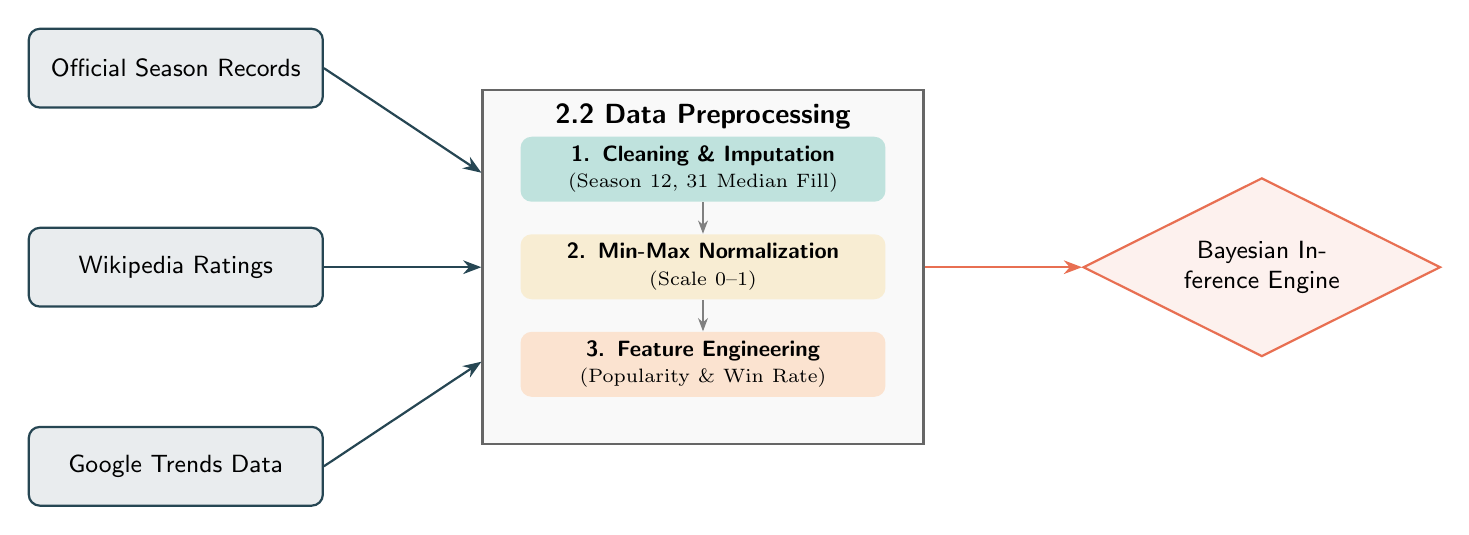
\begin{tikzpicture}[
    node distance=1.5cm and 2cm,
    font=\sffamily\small,
    % 样式定义
    source/.style={rectangle, rounded corners, draw=color1, fill=color1!10, thick, text width=3.5cm, align=center, minimum height=1cm},
    process/.style={rectangle, draw=black!60, fill=gray!5, thick, text width=5cm, align=left, minimum height=4.5cm, inner sep=0.3cm},
    step/.style n args={1}{rectangle, rounded corners, draw=none, text width=4.4cm, minimum height=0.8cm, align=center, font=\sffamily\bfseries\footnotesize},
    output/.style={diamond, aspect=2, draw=color5, fill=color5!10, thick, text width=2.5cm, align=center}
]

    % --- 左侧数据源 ---
    \node (src1) [source] {Official Season Records};
    \node (src2) [source, below=of src1] {Wikipedia Ratings};
    \node (src3) [source, below=of src2] {Google Trends Data};

    % --- 中间主框 ---
    \node (main) [process, right=of src2] {};
    \node at (main.north) [below=2pt, font=\sffamily\bfseries] {2.2 Data Preprocessing};
    
    % 内部步骤
    \node (s1) [rectangle, rounded corners, draw=none, text width=4.4cm, minimum height=0.8cm, align=center, font=\sffamily\bfseries\footnotesize, fill=color2!30, below=0.6cm of main.north] {1. Cleaning \& Imputation \\ \normalfont\scriptsize (Season 12, 31 Median Fill)};
    \node (s2) [rectangle, rounded corners, draw=none, text width=4.4cm, minimum height=0.8cm, align=center, font=\sffamily\bfseries\footnotesize, fill=color3!30, below=0.4cm of s1] {2. Min-Max Normalization \\ \normalfont\scriptsize (Scale 0--1)};
    \node (s3) [rectangle, rounded corners, draw=none, text width=4.4cm, minimum height=0.8cm, align=center, font=\sffamily\bfseries\footnotesize, fill=color4!30, below=0.4cm of s2] {3. Feature Engineering \\ \normalfont\scriptsize (Popularity \& Win Rate)};

    % --- 右侧输出 ---
    \node (out) [output, right=of main] {Bayesian Inference Engine};

    % --- 连线 ---
    \draw [-{Stealth}, thick, color1] (src1.east) -- ([yshift=1.2cm]main.west);
    \draw [-{Stealth}, thick, color1] (src2.east) -- (main.west);
    \draw [-{Stealth}, thick, color1] (src3.east) -- ([yshift=-1.2cm]main.west);
    
    \draw [-{Stealth}, thick, color5] (main.east) -- (out.west);
    
    % 内部小箭头
    \draw [-{Stealth}, gray] (s1) -- (s2);
    \draw [-{Stealth}, gray] (s2) -- (s3);

\end{tikzpicture}
\end{document}